\documentclass[10pt]{article}
\usepackage[preprint]{tmlr}

\input{math_commands.tex}

\usepackage{amsmath,amssymb}
\usepackage{booktabs}
\usepackage{enumitem}
\usepackage{float}
\usepackage{graphicx}
\usepackage{microtype}
\usepackage{tabularx}
\usepackage{tikz}
\usetikzlibrary{arrows.meta,fit,positioning,shapes.geometric}
\usepackage{xcolor}
\usepackage{hyperref}
\usepackage{url}
\usepackage{xspace}

\definecolor{unirlblue}{HTML}{2D5B9A}
\definecolor{unirlcyan}{HTML}{DCEEF7}
\definecolor{unirlgreen}{HTML}{DCEEDC}
\definecolor{unirlorange}{HTML}{FBE6C5}
\definecolor{unirlgray}{HTML}{EEF1F4}
\definecolor{todored}{HTML}{A52222}

\hypersetup{
  colorlinks=true,
  linkcolor=unirlblue,
  citecolor=unirlblue,
  urlcolor=unirlblue
}
\setlength{\emergencystretch}{2em}
\setlist[itemize]{leftmargin=*,topsep=2pt,itemsep=2pt}
\setlist[enumerate]{leftmargin=*,topsep=2pt,itemsep=2pt}

\newcommand{\system}{\textsc{UniRL}\xspace}
\newcommand{\sample}{\texttt{Sample}}
\newcommand{\parttype}{\texttt{Part}}
\newcommand{\paperTODO}[1]{\textcolor{todored}{\textbf{TODO[data]:} #1}}
\newcommand{\codepath}[1]{\texttt{#1}}
\newcolumntype{Y}{>{\raggedright\arraybackslash}X}
\newcolumntype{L}[1]{>{\raggedright\arraybackslash}p{#1}}

\title{\system: Trajectory-Centric Post-Training\\
Across Heterogeneous Generative Models}

\author{\name UniRL Authors \email authors@to.be.added \\
      \addr Affiliations to be added before the arXiv release}

\def\month{08}
\def\year{2026}
\def\openreview{\url{https://openreview.net/forum?id=to-be-assigned}}

\begin{document}

\maketitle

\begin{abstract}
Reinforcement-learning post-training systems are commonly organized around the same outer loop---generate, score, assign credit, and update---yet their implementations fragment along a second axis: autoregressive tokens, diffusion trajectories, multimodal values, and multi-stage or tool-interacting rollouts carry different state and impose different execution constraints.
We present \system, a trajectory-centric system that places a lineage-preserving, modality-aware intermediate representation at the boundary between post-training semantics and distributed execution.
A trajectory is an ordered tree of typed parts carrying user-visible values, model-facing conditions, optimization-facing segments, rewards, and the policy version that produced each generated frontier.
Rollout engines implement one transformation, $\sample\!\rightarrow\!\sample$, while logical roles, placement, tensor transport, weight publication, and phase residency determine how the transformation executes.
The same contracts therefore describe autoregressive, diffusion, composed, and tool-interacting workflows under colocated, disaggregated, synchronous, or bounded-staleness schedules, without asserting that their model-specific replay mathematics are identical.
This manuscript derives the design from UniRL commit \texttt{f5d7104} and specifies a claim-aligned evaluation covering training reproducibility, end-to-end throughput, phase cost, scaling, memory, transport, and policy lag.
A source-importing CPU harness already exercises ten core IR invariants and records preliminary container-operation costs; the multi-seed training and aligned GPU systems results remain open.
\paperTODO{Add artifact-backed headline findings only after the RQ1, RQ2, and RQ4 experiments in Section~\ref{sec:evaluation} are complete.}
\end{abstract}

\section{Introduction}
\label{sec:introduction}

Online post-training is a feedback program.
It expands inputs into policy samples, evaluates those samples, turns feedback into a learning signal, and applies one or more optimizer updates.
At this level, language-model GRPO, diffusion-model policy gradients, prompt-rewrite pipelines, and tool-using agents look deceptively similar.
Their data paths do not.
An autoregressive update may need packed token IDs, masks, rollout log probabilities, and per-token values; a diffusion update may need a sparse set of latent states, a noise schedule, and transition statistics; a composed workflow must retain which image descended from which rewritten prompt; an asynchronous run must additionally retain which policy version generated every sample.

Existing systems have made major progress on scalable LLM post-training and flexible device mapping~\citep{sheng2024hybridflow,hu2024openrlhf,wang2025roll,nemorl2025}.
Fully or partially asynchronous systems address rollout tail latency and accelerator idle time~\citep{fu2025areal,zhang2026relax,slime2025}.
Meanwhile, diffusion RL methods and multimodal frameworks broaden the optimization and model families that can be trained~\citep{black2023ddpo,liu2025flowgrpo,xue2025dancegrpo,zheng2025diffusionnft,verlomni2026}.
These advances also raise the bar for a new system paper: supporting more modalities or adding an asynchronous loop is not, by itself, a sufficient technical thesis.

\system starts from a narrower question:

\begin{quote}
\emph{Can one post-training program cross generative model families and execution topologies without discarding the structural information needed for correct grouping, replay, credit assignment, transport, and policy-version control?}
\end{quote}

Its answer is a trajectory intermediate representation (IR).
The IR makes a complete prompt-rooted lineage, rather than an individual row or an LLM-specific tensor dictionary, the unit of scheduling and sharding.
Typed leaves distinguish decoded multimodal values from model conditions and optimization segments.
Distributed methods declare how each structured field scatters, concatenates, packs, or remains shared.
Dense tensors can be replaced by row-addressable references without changing the trajectory structure.
This representation is passed through a small set of logical roles and can be mapped to colocated or disjoint GPU slabs.

The paper makes the following source-backed design contributions and turns each into a falsifiable empirical claim:

\begin{itemize}
  \item A \emph{lineage-preserving trajectory IR} for branching AR, diffusion, composed, and environment-interacting rollouts (Section~\ref{sec:trajectory}).  The empirical claim is not merely that these paths compile, but that the IR preserves grouping, replay state, and credit under real executions and a held-out integration.
  \item A \emph{separation between semantic roles and physical execution}: rollout remains $\sample\!\rightarrow\!\sample$, while placement, dispatch, tensor transport, weight publication, and residency are selected independently where their contracts permit (Section~\ref{sec:execution}).  The corresponding experiment runs matched work under multiple topologies.
  \item A \emph{version-aware scheduling discipline} shared by autoregressive and diffusion trainers.  It dynamically fills rollout lanes, but publishes weights only at a quiescent, batch-aligned boundary and filters samples by explicit policy lag (Section~\ref{sec:async}).  The corresponding experiment measures throughput--staleness--quality trade-offs.
  \item An evaluation protocol that separates \emph{training validity} from \emph{systems efficiency}, requires aligned effective work, and reports raw artifacts rather than undocumented benchmark prose (Section~\ref{sec:evaluation}).
\end{itemize}

The current manuscript intentionally contains no end-to-end training or systems-performance claim: the audited repository contains runnable instrumentation and comparison scripts but not the raw logs needed to verify prose-reported numbers.
We report only a narrowly scoped, artifact-backed CPU regression of IR operations in RQ3.
This evidence boundary prevents an implementation survey from masquerading as an evaluated systems result.

\section{Problem: Preserve Semantics While Changing Execution}
\label{sec:problem}

Let an online post-training iteration consume a batch of roots $X$, sample trajectories with behavior policy $\pi_v$, obtain reward $r$, construct credit $A$, and update parameters $\theta$:
\begin{equation}
X \xrightarrow{\pi_v} \mathcal{T}
  \xrightarrow{R} (\mathcal{T},r)
  \xrightarrow{C} (\mathcal{T},A)
  \xrightarrow{U_\theta} \theta'.
\label{eq:outer-loop}
\end{equation}
The compact notation hides three forms of heterogeneity.

\paragraph{Trajectory heterogeneity.}
The sufficient statistics for an update depend on the generative process.
For AR policies, a segment may be a variable-length packed token sequence with masks, old log probabilities, values, and returns.
For stochastic diffusion or flow policies, a segment may contain selected latent snapshots, a shared noise schedule, the indices of sampled transitions, and rollout or replay transition statistics.
Multi-stage and agentic paths add nonuniform lineage and observations.

\paragraph{Role heterogeneity.}
Generation, reward evaluation, model replay, gradient computation, and policy publication have different dependencies and may use distinct runtime systems.
Serving engines such as vLLM~\citep{kwon2023vllm} and SGLang~\citep{zheng2024sglang} are optimized for generation, while FSDP~\citep{zhao2023fsdp} or another training backend owns parameters and optimizer state.
Moving a large policy or trajectory between them is a first-order cost.

\paragraph{Topology heterogeneity.}
A small run may time-share one GPU set between training and rollout; a larger run may separate them; a variable-duration rollout may benefit from asynchronous admission.
Each choice changes memory pressure, transfer paths, synchronization frequency, and allowable policy lag.

These observations produce four requirements.

\begin{table}[H]
\caption{Design requirements and the corresponding UniRL mechanism. The right column states what must be evaluated; it is not a result.}
\label{tab:requirements}
\centering
\small
\begin{tabularx}{\textwidth}{@{}L{0.17\textwidth}Y Y@{}}
\toprule
Requirement & Mechanism & Evidence required \\
\midrule
Preserve structure & Parent-addressed parts; root-complete split, select, concat, and reward propagation & Trace invariants across AR, diffusion, and cross-stage runs \\
Preserve model state & Typed primitives, conditions, and AR/latent replay segments & Rollout--replay consistency and held-out integration \\
Change execution safely & Logical roles, placement scopes, field-aware dispatch, and tensor references & Matched-work topology and transport ablations \\
Control policy age & Version-stamped generated parts, lag filters, quiescent publication, and hard boundaries & Lag distributions, throughput, and time-to-quality \\
\bottomrule
\end{tabularx}
\end{table}

\paragraph{Non-goals.}
\system does not erase model-specific code: a model bundle still exposes architecture-specific stages, and an algorithm still defines its replay and loss.
It does not automatically discover an optimal placement.
The present runtime uses a driver to sequence roles and Ray actors~\citep{moritz2018ray} to host them; it is not a new cluster scheduler.
Finally, source-code breadth is not evidence that all combinations are production-ready.

\section{A Trajectory-Centric Programming Model}
\label{sec:trajectory}

\subsection{A trajectory is an ordered tree of parts}

The central type is
\begin{equation}
\mathcal{T} = [P_0,P_1,\ldots,P_L],
\qquad
P_i = (I_i, X_i, C_i, Z_i, R_i, A_i, V_i, M_i),
\label{eq:sample}
\end{equation}
where $I_i$ are sample identifiers, $X_i$ decoded modality values, $C_i$ model conditions, $Z_i$ optimization segments, $R_i$ rewards, $A_i$ advantages or returns, $V_i$ a behavior-policy version, and $M_i$ auxiliary metadata.
In code, $\mathcal{T}$ is a \sample{} and each $P_i$ is a \parttype{}.

Identifiers encode ancestry.
Root IDs contain no lineage separator; a branch appends a child ordinal.
For every non-root row $j$ in $P_i$, its parent ID must occur in $P_{i-1}$:
\begin{equation}
\forall i>0,\;\forall s\in I_i:\quad \operatorname{parent}(s)\in I_{i-1}.
\label{eq:parent-invariant}
\end{equation}
The constructor checks Equation~\ref{eq:parent-invariant}.
The \texttt{fork} operator appends $k$ generated children per frontier row; \texttt{observe} appends a branch-one input from an environment; and \texttt{propagate\_rewards} reduces child reward to an unscored parent.

Batch operations act on complete root groups.
\texttt{Sample.split()} returns one tree-complete trajectory per root, and slicing or selection is implemented by selecting these groups rather than independent rows.
Consequently, group-relative advantages and cross-stage credit do not depend on an incidental flat-row ordering after a distributed shuffle.

\begin{figure}[H]
\centering
\resizebox{0.98\textwidth}{!}{%
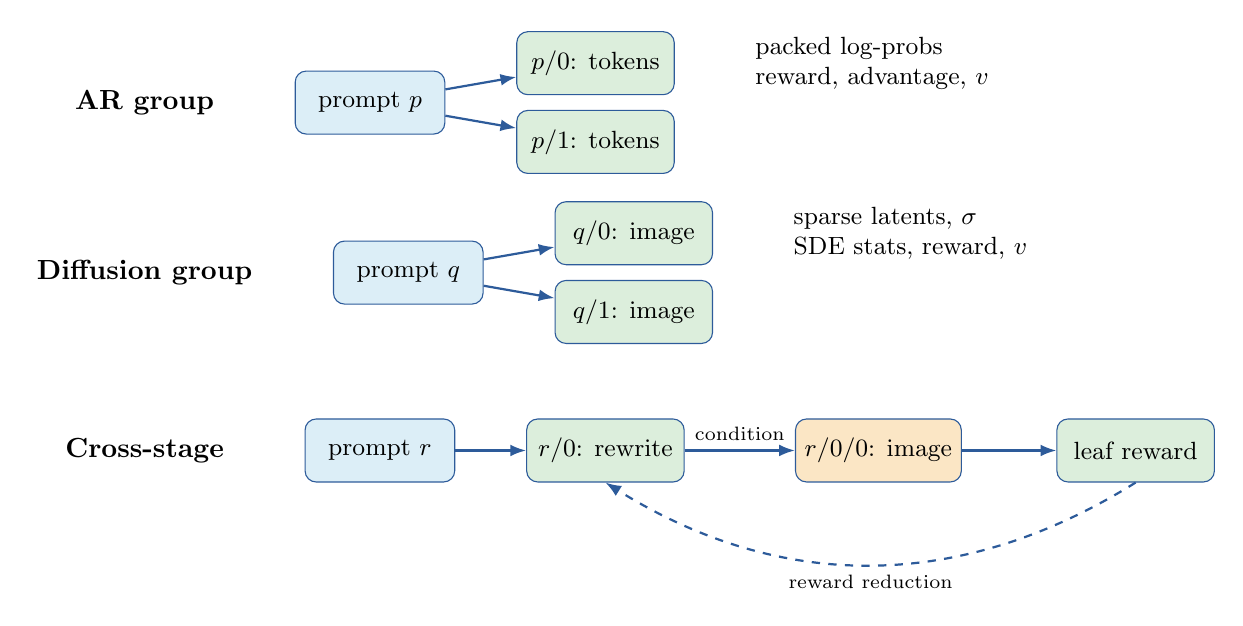
\begin{tikzpicture}[
  node distance=5mm and 9mm,
  every node/.style={font=\small},
  root/.style={draw=unirlblue,rounded corners,fill=unirlcyan,minimum width=19mm,minimum height=8mm},
  gen/.style={draw=unirlblue,rounded corners,fill=unirlgreen,minimum width=20mm,minimum height=8mm},
  obs/.style={draw=unirlblue,rounded corners,fill=unirlorange,minimum width=20mm,minimum height=8mm},
  arr/.style={-{Latex[length=2mm]},thick,draw=unirlblue}
]
\node[font=\bfseries] (arlabel) {AR group};
\node[root,right=of arlabel] (arp) {prompt $p$};
\node[gen,right=of arp,yshift=5mm] (ar0) {$p/0$: tokens};
\node[gen,right=of arp,yshift=-5mm] (ar1) {$p/1$: tokens};
\draw[arr] (arp) -- (ar0);
\draw[arr] (arp) -- (ar1);
\node[right=of ar0,align=left] {packed log-probs\\reward, advantage, $v$};

\node[font=\bfseries,below=16mm of arlabel] (dlabel) {Diffusion group};
\node[root,right=of dlabel] (dp) {prompt $q$};
\node[gen,right=of dp,yshift=5mm] (d0) {$q/0$: image};
\node[gen,right=of dp,yshift=-5mm] (d1) {$q/1$: image};
\draw[arr] (dp) -- (d0);
\draw[arr] (dp) -- (d1);
\node[right=of d0,align=left] {sparse latents, $\sigma$\\SDE stats, reward, $v$};

\node[font=\bfseries,below=17mm of dlabel] (clabel) {Cross-stage};
\node[root,right=of clabel] (cp) {prompt $r$};
\node[gen,right=of cp] (rewrite) {$r/0$: rewrite};
\node[obs,right=14mm of rewrite] (image) {$r/0/0$: image};
\node[gen,right=12mm of image] (credit) {leaf reward};
\draw[arr] (cp) -- (rewrite);
\draw[arr] (rewrite) -- node[above,font=\scriptsize]{condition} (image);
\draw[arr] (image) -- (credit);
\draw[arr,dashed,bend left=32] (credit.south) to node[below,font=\scriptsize]{reward reduction} (rewrite.south);
\end{tikzpicture}}
\caption{Three trajectory shapes represented by the same ordered-part IR. A generated part retains decoded values and the optimization segment required to replay its policy. The policy version $v$ is attached to generated frontiers. This diagram is reconstructed from current types and execution paths, not from the repository's legacy figures.}
\label{fig:trajectory-ir}
\end{figure}

\subsection{Values, conditions, and segments are separate layers}

\system distinguishes three kinds of leaves that are often conflated.

\paragraph{Primitives.}
Primitives are decoded or externally supplied values: text, images, videos, audio waveforms, and media references.
Image pixels and variable-duration video/audio values use packed representations with per-example shapes or cumulative offsets.
They are suitable for reward functions, visualization, and subsequent turns, but need not be the tensors replayed by the trainable model.

\paragraph{Conditions.}
Conditions are model-facing encodings, such as text embeddings or image latents.
They allow rollout adapters and train-side stages to agree on typed inputs without prescribing one tokenizer, text encoder, or multimodal fusion architecture.

\paragraph{Segments.}
Segments retain optimization-facing state.
\texttt{TextSegment} stores variable-length packed token fields.
\texttt{LatentSegment} stores latent snapshots at selected indices, a shared sigma schedule, and optional SDE log probabilities or transition means.
The sparse index map is important: a diffusion algorithm can replay only selected transitions instead of materializing an entire denoising path for every loss.

The distinction makes decoded payload lifetime independent of replay lifetime.
After reward logging, trainers may drop large decoded media while retaining conditions, segments, reward, and credit for training.

\subsection{A field algebra defines structural batching}

Every structured batch field declares a composition rule: concatenated, packed variable-length, shared, or reduced by maximum, minimum, sum, or mean.
These annotations drive concat, split, selection, repetition, and device movement recursively.
They also define how a distributed method reconstructs its return value.
For example, a DP-scattered rollout receives a tree-complete shard and returns parts that are merged position-wise; a broadcast lifecycle method returns one replicated control result.

This is a stronger contract than requiring each role to hand-author tensor slicing.
It also creates a measurable cost: recursive structural operations and reference bookkeeping must be benchmarked in Section~\ref{sec:rq3} rather than assumed free.

\subsection{Rollout engines implement one transformation}

Every rollout engine fills a request and returns a trajectory:
\begin{equation}
F_{\theta,e}: \mathcal{T}_{\mathrm{request}} \longrightarrow \mathcal{T}_{\mathrm{filled}},
\label{eq:engine}
\end{equation}
where $e$ identifies a train-side or external generation runtime.
The base contract also exposes lifecycle and policy-publication operations, but it does not standardize the engine's internal serving API.

The current source contains four useful forms of Equation~\ref{eq:engine}.
The train-side adapter invokes the model pipeline directly under evaluation mode.
Dedicated SGLang and vLLM-Omni adapters translate typed trajectory inputs to their native requests and rebuild typed responses.
A composed engine serially fills multiple generated parts, for example an AR rewrite followed by diffusion generation.
An agentic engine repeatedly appends policy turns and environment observations.
The claim is therefore about a common boundary, not one universal generation kernel.

\subsection{The algorithm boundary preserves specialized replay}

A train stack owns microbatch planning, gradient accumulation, global loss normalization, gradient clipping, optimizer steps, and per-update aggregation.
An algorithm object owns the stage-specific map
\begin{equation}
(C,Z,A;\theta) \longmapsto \mathcal{L}\quad\text{and backward}.
\label{eq:algorithm}
\end{equation}
Before repeated optimizer updates, the stack can freeze an old-policy anchor at the same microbatch geometry used for training.
AR objectives replay token log probabilities; diffusion objectives replay selected transitions and may compare rollout statistics, a pre-update replay, or a reference model.
Supervised and forward-process objectives explicitly opt out of advantages.

This division is deliberately not advertised as algorithmic novelty.
GRPO follows the group-relative formulation introduced for language reasoning~\citep{shao2024deepseekmath}; PPO follows proximal policy optimization~\citep{schulman2017ppo}; diffusion objectives build on prior diffusion-RL methods~\citep{black2023ddpo,liu2025flowgrpo,xue2025dancegrpo,zheng2025diffusionnft}.
The systems question is whether these objectives can consume the same trajectory and execution contracts without hiding their different sufficient statistics.

\section{From a Program to a Distributed Execution}
\label{sec:execution}

Figure~\ref{fig:architecture} separates the feedback program from the mechanisms that execute it.

\begin{figure}[H]
\centering
\resizebox{\textwidth}{!}{%
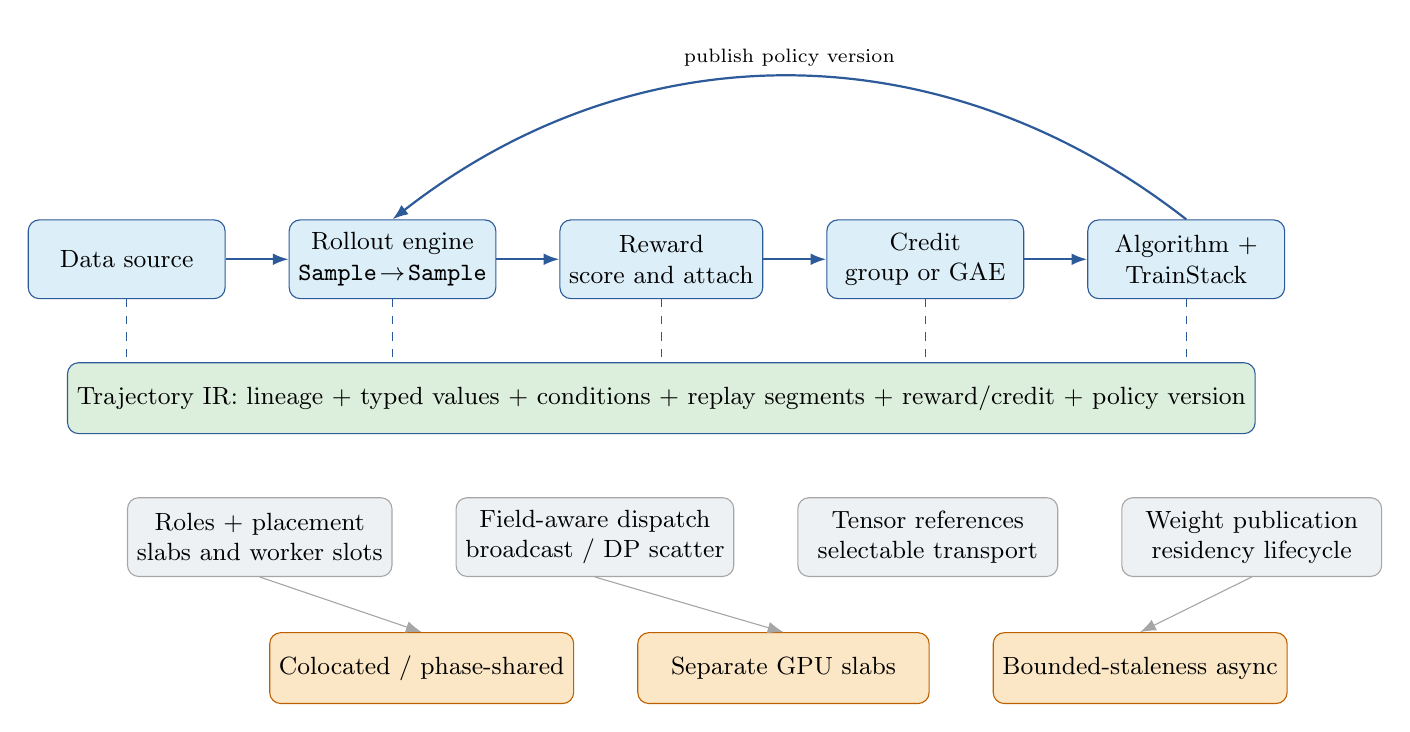
\begin{tikzpicture}[
  every node/.style={font=\small},
  role/.style={draw=unirlblue,rounded corners,fill=unirlcyan,minimum width=25mm,minimum height=10mm,align=center},
  ir/.style={draw=unirlblue,rounded corners,fill=unirlgreen,minimum height=9mm,align=center},
  mech/.style={draw=gray!70,rounded corners,fill=unirlgray,minimum width=33mm,minimum height=10mm,align=center},
  topo/.style={draw=orange!75!black,rounded corners,fill=unirlorange,minimum width=37mm,minimum height=9mm,align=center},
  arr/.style={-{Latex[length=2mm]},thick,draw=unirlblue}
]
\node[role] (data) {Data source};
\node[role,right=8mm of data] (rollout) {Rollout engine\\$\sample\!\rightarrow\!\sample$};
\node[role,right=8mm of rollout] (reward) {Reward\\score and attach};
\node[role,right=8mm of reward] (credit) {Credit\\group or GAE};
\node[role,right=8mm of credit] (train) {Algorithm +\\TrainStack};
\draw[arr] (data) -- (rollout);
\draw[arr] (rollout) -- (reward);
\draw[arr] (reward) -- (credit);
\draw[arr] (credit) -- (train);
\draw[arr,bend right=38] (train.north) to node[above,font=\scriptsize]{publish policy version} (rollout.north);

\node[ir,below=8mm of reward,minimum width=132mm] (irbar) {Trajectory IR: lineage $+$ typed values $+$ conditions $+$ replay segments $+$ reward/credit $+$ policy version};
\draw[dashed,draw=unirlblue] (data.south) -- (data.south |- irbar.north);
\draw[dashed,draw=unirlblue] (rollout.south) -- (rollout.south |- irbar.north);
\draw[dashed,draw=unirlblue] (reward.south) -- (reward.south |- irbar.north);
\draw[dashed,draw=unirlblue] (credit.south) -- (credit.south |- irbar.north);
\draw[dashed,draw=unirlblue] (train.south) -- (train.south |- irbar.north);

\node[mech,below=8mm of irbar,xshift=-51mm] (place) {Roles + placement\\slabs and worker slots};
\node[mech,right=8mm of place] (dispatch) {Field-aware dispatch\\broadcast / DP scatter};
\node[mech,right=8mm of dispatch] (transport) {Tensor references\\selectable transport};
\node[mech,right=8mm of transport] (lifecycle) {Weight publication\\residency lifecycle};

\node[topo,below=7mm of dispatch,xshift=-22mm] (coloc) {Colocated / phase-shared};
\node[topo,right=8mm of coloc] (separate) {Separate GPU slabs};
\node[topo,right=8mm of separate] (async) {Bounded-staleness async};
\draw[-{Latex[length=2mm]},draw=gray!70] (place.south) -- (coloc.north);
\draw[-{Latex[length=2mm]},draw=gray!70] (dispatch.south) -- (separate.north);
\draw[-{Latex[length=2mm]},draw=gray!70] (lifecycle.south) -- (async.north);
\end{tikzpicture}}
\caption{Source-derived UniRL architecture. The top row is the feedback program; the green bar is its stable data boundary. The lower rows map logical roles to communication and resource policies. Not every topology is valid for every engine; startup validation rejects unsupported combinations.}
\label{fig:architecture}
\end{figure}

\subsection{Logical roles, device slabs, and worker slots}

A \texttt{DevicePool} creates one Ray worker per GPU initially and reserves one strict-packed placement group per node.
A placement scope selects a fraction of currently available devices.
Roles created inside a scope either share its worker slot---enabling local sibling access and memory time-sharing---or receive isolated slots on the same devices.
Disjoint top-level scopes form separate training, rollout, or reward slabs.

A role is a regular Python object derived from \texttt{Remote}.
The handle constructs one role replica on each selected worker and derives data-, tensor-, pipeline-, sequence-, and expert-parallel rank metadata from the role configuration.
Method decorators state argument dispatch and return collection.
The trainer is consequently a single-controller program, while each method may invoke multi-controller distributed training or serving inside a role.
This resembles HybridFlow's separation between orchestration and distributed computation~\citep{sheng2024hybridflow}; UniRL's paper claim centers instead on carrying the same typed lineage through heterogeneous generative stages.

\subsection{Tensor references decouple structure from movement}

Before an RPC, dense tensor leaves may be \emph{dehydrated} into \texttt{TensorRef}s.
A reference is an ordered list of half-open row spans over opaque handles, plus shape, dtype, and device metadata.
Selection and contiguous slicing construct new span views without moving tensor data.
At a destination, hydration resolves all referenced spans in a batch and reconstructs the original nested object.

The transport interface has a deliberately small contract: store tensors, resolve handles, identify references, and optionally localize references for destination workers.
The audited source provides (i) a colocated per-worker store, (ii) a per-GPU store with IPC and NCCL transfers, and (iii) a TransferQueue path backed by simple storage or Mooncake-compatible storage.
Mooncake itself was proposed for disaggregated serving~\citep{qin2024mooncake}; here its storage interface is a transport option rather than a claimed UniRL invention.

The driver can therefore manipulate trajectory structure and metadata without materializing all GPU tensors.
Whether this reduces memory and transfer cost in practice is RQ3, not an assumption.

\subsection{Phase lifecycles and policy publication}
\label{sec:lifecycle}

Training and generation often hold different copies or formats of a policy.
UniRL exposes their interaction as an ordered lifecycle:
\begin{enumerate}
  \item wake the rollout engine sufficiently to receive weights;
  \item publish parameters if the cadence requires it;
  \item optionally offload colocated training state;
  \item generate and stamp the frontier with the engine's policy version;
  \item sleep the engine when the selected residency policy requires it;
  \item restore training state before replay and optimization.
\end{enumerate}

The concrete order varies by engine capabilities.
For example, staged wake can receive weights before mapping the rest of an AR engine, and a train-side engine reads live model objects without a separate publication role.
Separate slabs use an explicit one-time handshake.
Weight-sync implementations cover LoRA tensor paths and several full-weight paths, including tensor serialization, CUDA IPC, NCCL, and checkpoint rendezvous.
The base engine can also receive per-track updates for composed models.

The source rejects combinations whose lifecycle has not been validated, such as a train-side rollout on a physically separate slab or selected EMA/offload combinations.
This fail-closed policy is important because a partially awakened engine or silently stale adapter can produce plausible but invalid training data.
Section~\ref{sec:evaluation} therefore includes replay-consistency and failure-injection checks alongside throughput.

\subsection{Synchronous execution}

The synchronous AR trainer performs rollout, reward, credit assignment, replay/update, optional evaluation, and checkpointing in order.
The diffusion trainer can accumulate multiple rollouts into one optimizer window and can place reward on the train slab or a third slab.
In both cases, topology affects resource ownership and residency but not the trajectory boundary.
This makes a controlled topology experiment possible: hold model, prompts, group size, reward, number of replayed steps or tokens, and optimizer updates constant while changing only engine or placement.

\subsection{Bounded-staleness execution}
\label{sec:async}

Asynchrony changes correctness conditions, not just control flow.
UniRL's asynchronous AR and diffusion trainers share one manager.
A background dispatcher fills every engine slot up to a configured per-worker capacity.
Completed trajectories are grouped by root; only complete groups enter the ready buffer.
Every generated part must carry an output policy version $v_o$.

Let $v_t$ be the current optimizer-update version and $u$ the number of optimizer updates performed per consumed rollout batch.
The manager exposes lag in update units,
\begin{equation}
\ell = v_t-v_o,
\end{equation}
and filters completed work against a configured budget.
Before publishing version $v_t$, it pauses admission, drains or suspends work, completes any started or batch-aligning prefix, checks that no publication splits a training batch across behavior versions, publishes weights, updates the rollout version, and then resubmits eligible pristine carry.
Evaluation and checkpointing require a fully empty manager.

This discipline differs from claiming fully asynchronous optimization.
Weight publication remains a barrier, and the current asynchronous diffusion path deliberately limits in-flight batch structure more tightly than the AR path.
The evaluation must report the actual lag histogram, dropped work, and barrier time; a nominal ``async'' label is insufficient.

\section{Instantiations of the Common Contracts}
\label{sec:instantiations}

This section illustrates why the trajectory boundary is useful; it is not a support matrix.

\subsection{Autoregressive reasoning}

An input part carries prompt text and metadata.
Forking by group size creates generated shells with sibling IDs.
An AR engine fills packed token segments and decoded text, a reward role attaches scalar or component rewards, and the part computes group-normalized credit or token-level generalized advantage estimates.
The train stack replays the same segment and applies the selected objective.
Optional token-length balancing permutes complete samples before DP sharding, preserving sibling identifiers and precomputed credit.

\subsection{Diffusion and flow generation}

A diffusion request forks prompts and records sampling parameters, a sigma schedule, selected SDE indices, and an initial-noise recipe.
The engine returns decoded media plus a latent segment whose sparse trajectory fields are sufficient for the selected update.
FlowGRPO-style objectives replay recorded steps and compare new transition log probabilities against a frozen rollout or replay anchor~\citep{liu2025flowgrpo}.
Forward-process objectives such as DiffusionNFT use clean generated samples rather than the same reverse-trajectory likelihood path~\citep{zheng2025diffusionnft}.
The common train stack handles microbatching and optimizer state; the algorithm remains responsible for these incompatible estimators.

\subsection{Cross-stage and environment-interacting trajectories}

In a prompt-enhancement path, one root produces one or more AR rewrites, and every rewrite produces one or more images.
The image reward is attached to the leaf and reduced to the rewrite parent before updating the relevant stage.
In a tool-interacting path, the policy emits an action-like text part, the environment appends an observation part, and the process repeats until termination or suspension.
Both workflows need ancestry to survive rollout scheduling and sharding; flattening them into unrelated rows would require rebuilding that correspondence out of band.

The decisive experiment is a held-out cross-stage integration and a lineage-breaking ablation, not the number of in-tree adapters.

\section{Evaluation Plan}
\label{sec:evaluation}

We organize evaluation around four research questions.
Each reported run must archive the resolved configuration, commit and dirty diff, model and dataset revisions, environment manifest, raw logs, structured metrics, parser version, and evaluation outputs.
Primary comparisons use the same hardware one framework at a time.

\subsection{RQ1: Does UniRL reproduce credible training behavior?}
\label{sec:rq1}

The first question is scientific rather than purely operational.
A successful run must exhibit reasonable learning dynamics and final task performance relative to the base policy and an aligned reference implementation.

\paragraph{AR workload.}
We will train a documented Qwen3-class checkpoint with GRPO on a fixed mathematical-reasoning dataset and evaluate frozen checkpoints on MATH-500 and AIME snapshots.
The UniRL run and the selected current reference must align prompts, chat template, verifier, maximum generation length, group size, effective batch, clipping, KL treatment, optimizer updates, and evaluation decoding.
We will report at least three seeds, reward and external-evaluation curves, final and best-checkpoint results, and confidence intervals.

\paragraph{Diffusion workload.}
We will train SD3.5-Medium or Qwen-Image with a FlowGRPO workload whose prompt set, resolution, denoising schedule, SDE window, LoRA targets, reward, and optimizer work can be reproduced in a current reference.
External evaluation includes GenEval-style compositional accuracy plus a quality/diversity guard metric so that reward improvement cannot alone establish success.
A second forward-process objective is included only if its reference can be aligned without changing the paper's central systems question.

\paragraph{Cross-stage workload.}
One prompt-rewrite--generation or tool-interaction run will serialize complete trajectories and demonstrate credit propagation.
This workload tests representation and integration, not necessarily state-of-the-art task quality.

\begin{table}[H]
\caption{Planned reproducibility matrix. Dashes are deliberately not numerical placeholders.}
\label{tab:rq1}
\centering
\small
\begin{tabularx}{\textwidth}{@{}lXllll@{}}
\toprule
Family & Workload & Base & Reference & UniRL & Seeds \\
\midrule
AR & Qwen3-class GRPO; math verifier; MATH-500/AIME & -- & -- & -- & $\geq3$ \\
Diffusion & SD3.5-M or Qwen-Image FlowGRPO; external image eval & -- & -- & -- & $\geq3$ \\
Cross-stage & AR rewrite $\rightarrow$ diffusion/tool outcome & -- & ablation & -- & $\geq3$ \\
\bottomrule
\end{tabularx}
\par\vspace{1mm}
\paperTODO{Populate with mean, uncertainty, exact checkpoint revisions, and released run IDs.}
\end{table}

\subsection{RQ2: What is end-to-end system performance?}
\label{sec:rq2}

The primary diffusion comparison is an aligned SD3.5 FlowGRPO pair against a pinned current VeRL-Omni checkout, the closest public framework in scope~\citep{verlomni2026}.
An AR comparison uses a current LLM RL system selected for reproducible semantic parity, such as veRL, NeMo-RL, or another maintained baseline.
For every pair we report two rows when possible: aligned backends and each system's documented best valid configuration.

Metrics include median, mean, and p90 iteration time after a prespecified warmup; samples/s and samples/GPU-hour; per-phase time for generation, reward, credit, anchor/replay, backward/optimizer, weight publication, wake/sleep, and barriers; peak allocated and reserved GPU memory by role; CPU memory; utilization; and GPU-hours to a fixed external-evaluation threshold.
Strong and weak scaling use fixed global and fixed per-GPU work, respectively.

\begin{table}[H]
\caption{Systems result schema. Every cell will be derived from archived raw artifacts.}
\label{tab:rq2}
\centering
\small
\begin{tabularx}{\textwidth}{@{}lXrrrrr@{}}
\toprule
System & Configuration & s/iter & samples/s & samples/GPU-h & peak GiB & time-to-quality \\
\midrule
UniRL & aligned backend & -- & -- & -- & -- & -- \\
Closest baseline & aligned backend & -- & -- & -- & -- & -- \\
UniRL & best valid config & -- & -- & -- & -- & -- \\
Closest baseline & best valid config & -- & -- & -- & -- & -- \\
\bottomrule
\end{tabularx}
\par\vspace{1mm}
\paperTODO{Run on identical hardware, disclose inherent stack-version differences, and include failed/retried iterations.}
\end{table}

\subsection{RQ3: What does the trajectory abstraction cost and enable?}
\label{sec:rq3}

We measure recursive IR operations and tensor transport separately from model compute.
Microbenchmarks vary root count, branch factor, number and size of tensor leaves, ragged token/media lengths, and part depth.
They report split/concat/select latency, reference metadata bytes, dense bytes avoided at the driver, same-GPU and cross-GPU transfer time, cross-node time when available, and correctness hashes after reassembly.

End-to-end ablations compare the colocated store, per-GPU store, and TransferQueue path where the hardware supports them.
We also compare whole-tree sharding to a controlled flat-row handoff.
The latter must either rebuild lineage explicitly or expose the semantic error; it is not permitted to silently change group-relative credit.

The enablement test integrates one held-out model or cross-stage workflow.
We report which new bundle/stage/adapter code is required and which trainer, scheduler, transport, and credit code remains unchanged.
Changed lines are supporting evidence, not a standalone measure of quality.

\paragraph{Preliminary executable evidence.}
We ran a source-importing regression harness against a clean UniRL checkout at
\texttt{f5d7104}; it does not mock the trajectory classes.
All ten checks passed: cross-stage lineage construction, exact tree split/concat,
whole-tree select/slice, leaf-to-root reward propagation and group advantages,
rejection of malformed lineage and primitive modality/batch violations, variable-length packed-text
round trips, and lazy \texttt{TensorRef} selection/materialization including bounds
checking.
Table~\ref{tab:cpu-ir} reports a deliberately narrow timing slice from the same run.
The synthetic workload has four AR children per root, one observation per AR child,
two diffusion children per observation, and a four-value image payload per leaf.

\begin{table}[H]
\caption{Preliminary single-process CPU trajectory-IR timings (microseconds).
Python 3.12.14 and PyTorch 2.11.0; one thread; ten warm-up and 100 measured repetitions.
These are regression measurements, not distributed or GPU throughput.}
\label{tab:cpu-ir}
\centering
\scriptsize
% Generated by experiments/trajectory_ir/run_cpu_evidence.py; do not edit by hand.
\begin{tabular}{@{}rrlrr@{}}
\toprule
Roots & Leaf rows & Operation & Median & p90 \\
\midrule
8 & 64 & \texttt{sample.split\_concat} & 201.3 & 212.0 \\
8 & 64 & \texttt{sample.select\_half} & 954.2 & 977.7 \\
8 & 64 & \texttt{tensorref.select\_strided} & 20.1 & 20.4 \\
32 & 256 & \texttt{sample.split\_concat} & 488.6 & 496.8 \\
32 & 256 & \texttt{sample.select\_half} & 3538.6 & 3615.8 \\
32 & 256 & \texttt{tensorref.select\_strided} & 74.1 & 76.8 \\
128 & 1024 & \texttt{sample.split\_concat} & 1653.0 & 1700.5 \\
128 & 1024 & \texttt{sample.select\_half} & 13893.5 & 14139.3 \\
128 & 1024 & \texttt{tensorref.select\_strided} & 327.9 & 337.5 \\
\bottomrule
\end{tabular}

\end{table}

The current \texttt{Sample.select} path forms tree-complete root shards before
gathering them, so its cost grows with the full input tree rather than only the
selected rows. Strided \texttt{TensorRef} selection creates many metadata spans
while contiguous selection coalesces them; no dense tensor is copied until
materialization. These observations motivate, but do not replace, the planned
GPU transport and end-to-end ablations. The manifest, 100 per-cell raw trials,
structured check outcomes, generated table rows, and SHA-256 checksums are archived
under \codepath{artifacts/trajectory\_ir/cpu\_f5d7104\_macos\_arm64/}.

\subsection{RQ4: When is bounded-staleness execution useful?}
\label{sec:rq4}

We compare synchronous and asynchronous runs with identical effective optimizer work while sweeping generation-time variance, number of in-flight prompts, publication interval, and allowed lag.
Results include generation-latency distributions, engine occupancy, trainer idle fraction, publication/barrier time, completed and discarded samples, realized lag histograms, reward/eval versus optimizer update, and reward/eval versus wall time.
The key plot is a Pareto frontier of time-to-quality and realized policy lag.

\paragraph{A controlled pair does not yet exist in the stock recipes.}
At the audited commit, the nominal Qwen3 GRPO sync and async example files differ in five fields that affect either the estimator or learner execution (Table~\ref{tab:sync-async-preflight}).
Consequently, measurements from those files without overrides are inadmissible as evidence about asynchrony.
The GPU study will first choose one value for every controlled field, apply explicit overrides, archive both fully resolved Hydra configurations, and produce a field-by-field parity report.
Only topology, concurrency, publication interval, and allowed policy lag may then vary.

\begin{table}[H]
\caption{Mandatory preflight corrections for the stock Qwen3 GRPO sync/async pair at commit \texttt{f5d7104}. These are source/config observations, not results.}
\label{tab:sync-async-preflight}
\centering
\scriptsize
\begin{tabularx}{\textwidth}{@{}L{0.29\textwidth}YYL{0.30\textwidth}@{}}
\toprule
Controlled field & Sync stock & Async stock & Required action \\
\midrule
\texttt{normalize\_adv\_by\_std} & \texttt{true} & \texttt{false} & Match the advantage estimator. \\
High clipping bound & unset & \texttt{0.28} & Match symmetric/asymmetric clipping. \\
Loss aggregation & sequence mean, then token mean & sequence mean, token sum normalized & Match sequence-length weighting. \\
Attention implementation & \texttt{flex\_attention} & default & Match for backend-aligned rows. \\
Microplanner & token budget, 10,240 & default count planner & Match packing and learner work. \\
\bottomrule
\end{tabularx}
\end{table}

\paragraph{Measurement readiness.}
The current structured logger supplies end-to-end step time; six coarse phases (wake, generation, sleep, weight synchronization, reward, and aggregate training); rollout diagnostics; peak allocated/reserved GPU memory; and output, train, and published versions with realized lag.
Before RQ2 and RQ4, instrumentation must separate credit, replay/anchor, backward, optimizer, checkpoint, and publication-barrier time, and must emit complete per-step series for buffer occupancy and admitted, carried, suspended, rejected, discarded, retried, and completed work.
GPU utilization and power must be collected by an external monitor synchronized to the run clock.
Missing structured fields may not be reconstructed from isolated console messages or dashboard screenshots.

\begin{figure}[H]
\centering
\resizebox{0.94\textwidth}{!}{%
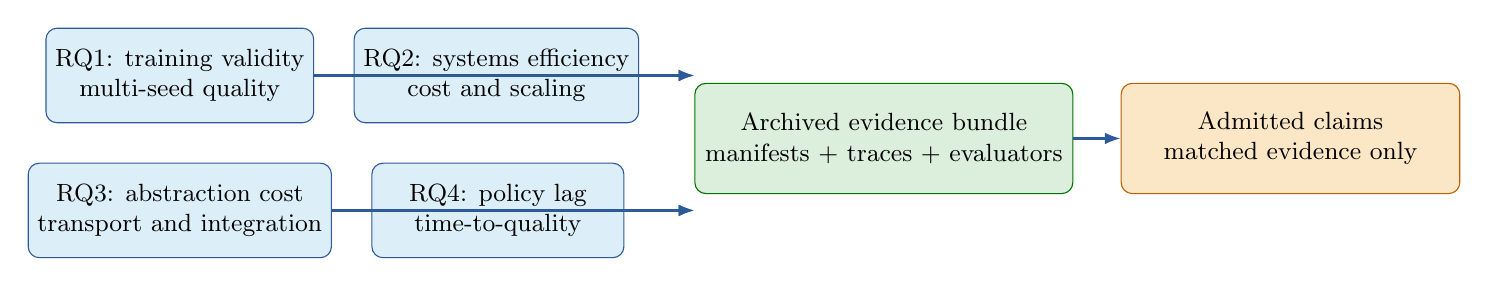
\begin{tikzpicture}[
  every node/.style={font=\small},
  rq/.style={draw=unirlblue,rounded corners,fill=unirlcyan,minimum width=32mm,minimum height=12mm,align=center},
  artifact/.style={draw=green!45!black,rounded corners,fill=unirlgreen,minimum width=48mm,minimum height=14mm,align=center},
  claim/.style={draw=orange!75!black,rounded corners,fill=unirlorange,minimum width=43mm,minimum height=14mm,align=center},
  arr/.style={-{Latex[length=2mm]},thick,draw=unirlblue}
]
\node[rq] (rq1) {RQ1: training validity\\multi-seed quality};
\node[rq,right=5mm of rq1] (rq2) {RQ2: systems efficiency\\cost and scaling};
\node[rq,below=5mm of rq1] (rq3) {RQ3: abstraction cost\\transport and integration};
\node[rq,right=5mm of rq3] (rq4) {RQ4: policy lag\\time-to-quality};
\node[artifact,right=7mm of rq2,yshift=-8mm] (artifact) {Archived evidence bundle\\manifests $+$ traces $+$ evaluators};
\node[claim,right=6mm of artifact] (claims) {Admitted claims\\matched evidence only};
\draw[arr] (rq1.east) -- (artifact.west |- rq1.east);
\draw[arr] (rq2.east) -- (artifact.west |- rq2.east);
\draw[arr] (rq3.east) -- (artifact.west |- rq3.east);
\draw[arr] (rq4.east) -- (artifact.west |- rq4.east);
\draw[arr] (artifact) -- (claims);
\end{tikzpicture}}
\caption{Claim-aligned evaluation contract. Scientific validity and systems efficiency are primary; mechanism costs and staleness explain when the design helps. Every quantitative claim must resolve to the same archived evidence bundle.}
\label{fig:evaluation-contract}
\end{figure}
\paperTODO{Add artifact-generated result panels for learning curves, phase breakdown, scaling and utilization, and the throughput--policy-lag Pareto frontier.}

\subsection{Fairness and statistical protocol}

Effective work is matched before wall-clock time: prompts, samples per prompt, decoded resolution or maximum tokens, rollout steps, replayed steps/tokens, microbatching semantics, and optimizer updates.
Reward placement is either identical and counted on both sides or excluded with a separate service-cost report.
We prespecify warmup removal, use at least 20 steady-state iterations for throughput summaries, and report the full distribution rather than a single minimum.
Training claims use independent seeds and external evaluation; time-to-quality uses the same evaluator and threshold.

\section{Related Work}
\label{sec:related}

\paragraph{LLM post-training systems.}
HybridFlow/veRL combines single- and multi-controller execution and introduces hierarchical APIs for mapping RLHF dataflows to devices~\citep{sheng2024hybridflow}.
OpenRLHF uses Ray, vLLM, and DeepSpeed to schedule the models in an RLHF workflow~\citep{hu2024openrlhf}.
ROLL emphasizes a single-controller abstraction, parallel workers, sample lifecycle scheduling, and flexible device mapping~\citep{wang2025roll}.
NeMo-RL provides scalable training and generation backends and multimodal model support~\citep{nemorl2025}.
UniRL shares their concern for composable orchestration; its intended distinction is the lineage- and modality-aware trajectory boundary across AR, diffusion, and cross-stage generation.
That distinction must be established by RQ3 rather than a feature table.

\paragraph{Asynchronous post-training.}
AReaL fully decouples generation and training and controls staleness to improve language-reasoning throughput~\citep{fu2025areal}.
Relax uses service-level separation, a TransferQueue data bus, and configurable staleness for omni-modal post-training~\citep{zhang2026relax}.
slime supports persistent asynchronous rollout generation around a training/rollout/data-buffer loop~\citep{slime2025}.
These systems make asynchrony an execution design space, not a UniRL novelty claim.
UniRL contributes a particular version-stamped group and publication-boundary discipline shared by AR and diffusion paths; RQ4 tests whether that discipline is useful.

\paragraph{Multimodal and diffusion post-training systems.}
VeRL-Omni extends veRL toward diffusion, unified, and omni-modality models and integrates vLLM-Omni rollout~\citep{verlomni2026}.
Relax is explicitly omni-native~\citep{zhang2026relax}.
Accordingly, ``supporting image, video, or audio'' cannot be the paper's contribution.
The comparison instead asks whether a single typed lineage simplifies cross-stage workflows and remains stable across execution modes.

\paragraph{Diffusion RL algorithms.}
DDPO casts denoising as a multi-step decision process~\citep{black2023ddpo}.
Flow-GRPO converts flow sampling to an SDE and applies group-relative optimization~\citep{liu2025flowgrpo}; DanceGRPO generalizes related ideas across visual generation tasks~\citep{xue2025dancegrpo}; DiffusionNFT instead optimizes a forward-process objective from reward-ranked generations~\citep{zheng2025diffusionnft}.
UniRL implements several algorithm families but does not claim their mathematical ideas.
Its algorithm interface keeps their incompatible replay state explicit while reusing scheduling and training mechanics.

\section{Limitations and Open Evidence}
\label{sec:limitations}

\paragraph{Integration is not automatic.}
Each new architecture still needs a bundle, stages, conditions, and adapters for the selected rollout runtime.
A common trajectory type does not eliminate tokenizer, scheduler, latent-layout, LoRA-target, or serving-version incompatibilities.

\paragraph{Topology is configured, not optimized.}
Placement scopes make resource choices explicit but do not search for the best split.
The best topology depends on model memory, reward cost, rollout variance, interconnect, and publication size.

\paragraph{Asynchronous execution is bounded and partially specialized.}
Publication is a barrier, and current AR and diffusion paths impose different admissible in-flight structure.
Fault isolation is limited by the shared Ray runtime and role lifecycle; the system does not yet claim service-level recovery comparable to dedicated service architectures.

\paragraph{The empirical case is incomplete.}
At the audited commit, raw logs sufficient to verify existing benchmark prose were absent from the checkout.
Therefore this draft makes no end-to-end throughput, scaling, memory, convergence, or final-quality claim.
Sections~\ref{sec:rq1}--\ref{sec:rq4} define the evidence required to remove this limitation.

\section{Conclusion}

\system treats post-training as a trajectory program whose semantic object survives changes in generative family and execution topology.
Lineage, typed modality values, replay segments, reward, credit, and policy version live in one IR; rollout, reward, training, transport, and publication are logical roles mapped separately to resources.
This design is most valuable if it passes two empirical tests: credible learning behavior across representative AR and diffusion workloads, and competitive end-to-end execution without weakening semantic parity.
The final paper will be complete only when the artifact-backed evaluation establishes both.

\section*{Reproducibility statement}

The source characterization in this draft refers to UniRL commit
{\small\texttt{f5d710406b215bb7a0b387fdd37e4d4778b92338}} (2026-08-20).
The manuscript repository records the claim-to-evidence plan in \texttt{PAPER\_PLAN.md}.
The cluster-ready execution protocol, configuration-parity gates, metric inventory,
and immutable run-directory contract are specified in
\texttt{EXPERIMENT\_RUNBOOK.md}; that document intentionally contains no results.
The preliminary RQ3 evidence is regenerated by
\codepath{experiments/trajectory\_ir/run\_cpu\_evidence.py}; its manifest pins the
source state, command, environment, workload, warm-up, repetitions, and timer.
\paperTODO{Before release, add the public artifact DOI/URL and author metadata, then archive manifests and regeneration scripts for every remaining result and figure.}

\bibliographystyle{tmlr}
\bibliography{main}

\appendix

\section{Claim-to-source audit}
\label{app:source-audit}

Table~\ref{tab:source-audit} records the executable source used to support mechanism descriptions.
It does not prove performance or successful execution for every configuration.

\begin{table}[H]
\caption{Primary code evidence at commit \texttt{f5d7104}.}
\label{tab:source-audit}
\centering
\scriptsize
\begin{tabularx}{\textwidth}{@{}L{0.20\textwidth}Y@{}}
\toprule
Mechanism & Primary source symbols \\
\midrule
Trajectory IR & \codepath{unirl/types/sample.py}: \texttt{Part}, \texttt{Sample}; \codepath{unirl/types/primitives.py}; \codepath{unirl/types/segments/} \\
Batch algebra & \codepath{unirl/distributed/tensor/batch.py}: \texttt{FieldKind}, \texttt{Batch} \\
Tensor references & \codepath{unirl/distributed/tensor/ref.py}: \texttt{TensorSpan}, \texttt{TensorRef}; \codepath{transport.py}: \texttt{TensorTransport} \\
Roles and placement & \codepath{unirl/distributed/group/device\_pool.py}, \codepath{placement.py}, \codepath{handle.py}, \codepath{dispatch.py} \\
Rollout boundary & \codepath{unirl/rollout/engine/base.py}: \texttt{BaseRolloutEngine}; concrete engines under \codepath{unirl/rollout/engine/} \\
Training boundary & \codepath{unirl/algorithms/base.py}: \texttt{StageAlgorithm}; \codepath{unirl/train/stack/base.py}: \texttt{TrainStack} \\
Sync trainers & \codepath{unirl/trainer/ar.py}: \texttt{ARTrainer}; \codepath{unirl/trainer/diffusion.py}: \texttt{DiffusionTrainer} \\
Async scheduler & \codepath{unirl/trainer/async\_rollout.py}; \codepath{unirl/rollout/manager/} \\
Weight publication & \codepath{unirl/distributed/weight\_sync/}; engine-specific receivers under \codepath{unirl/rollout/engine/} \\
Instrumentation & \codepath{unirl/utils/profiling.py}, \codepath{memory\_monitor.py}, \codepath{wandb\_logger.py} \\
\bottomrule
\end{tabularx}
\end{table}

\section{Required run artifact schema}
\label{app:artifacts}

Every result row must resolve to a run directory containing:
\begin{itemize}
  \item source and baseline commit hashes, submodule hashes, and dirty patches;
  \item the launch command and fully resolved configuration;
  \item model, reward, dataset, and tokenizer revisions or content hashes;
  \item GPU model/count, node/interconnect description, driver, CUDA, PyTorch, generation-engine, and training-backend versions;
  \item raw stdout/stderr, per-step structured timing, memory and utilization traces, checkpoint metadata, and evaluation outputs;
  \item seed, warmup exclusion rule, failure/retry accounting, and statistical aggregation script.
\end{itemize}

For training runs, serialized trace samples must redact private data while retaining lineage IDs, shapes, dtypes, policy versions, reward components, and segment index metadata.
For system baselines, an alignment manifest must explain every nonidentical setting and whether it changes effective work.

\section{Correctness status and remaining checks}
\label{app:correctness}

\paragraph{Executed locally.}
The preliminary RQ3 harness performs ten fail-fast checks on the audited source:
lineage-valid cross-stage construction; exact split/concat; tree-complete select and
slice; mean reward propagation plus group-normalized advantages; rejection of bad
lineage, modality keys, and primitive batch sizes; packed variable-length text
select/concat; and lazy tensor-reference selection, materialization, identity, and
bounds behavior. The structured outcomes and data-sensitive SHA-256 round-trip hash
are stored with the run artifacts.

\paragraph{Required before performance interpretation.}
The following system-level checks remain prerequisites for RQ1, RQ2, and RQ4:
\begin{enumerate}
  \item \textbf{Rollout--replay parity:} before the first update, compare engine-emitted and train-side replay log probabilities or transition statistics under stated numerical tolerances.
  \item \textbf{Publication parity:} repeat the parity check after each LoRA or full-weight publication path used in an experiment.
  \item \textbf{Batch-version integrity:} verify that an optimizer batch never mixes behavior versions when the configured algorithm assumes one version.
  \item \textbf{Boundary integrity:} checkpoint and evaluation begin only after the async manager is empty; resume restores the optimizer version and republishes it before new rollout.
  \item \textbf{Work accounting:} compare generated tokens or pixels, denoising and replay steps, scored samples, and committed optimizer updates across systems.
\end{enumerate}

\end{document}
